% Team paper draft. Layout approximates NeurIPS (5.5in x 9in text, Times, 10pt). For submission, switch to the official
% NeurIPS style: replace the geometry/font block below with \usepackage{neurips_20XX} from the course-linked template.
% Build: tectonic main.tex  (or pdflatex + bibtex in Overleaf). Figures come from `python state_bc/make_figures.py`.
\documentclass[10pt]{article}
\usepackage[letterpaper,textwidth=5.5in,textheight=9in,top=1in,headheight=12pt,headsep=25pt,footskip=30pt]{geometry}
\usepackage[T1]{fontenc}
\usepackage{amsmath}
\usepackage{newtxtext,newtxmath}  % provides the amssymb symbols; do not also load amssymb
\usepackage{booktabs}
\usepackage{graphicx}
\usepackage{xcolor}
\usepackage{algorithm}
\usepackage{algpseudocode}
\usepackage{microtype}
\usepackage{xurl}
\usepackage[hidelinks]{hyperref}
\emergencystretch=1.5em  % lets lines with long \texttt names break instead of running into the margin
\usepackage{natbib}
\setcitestyle{numbers,square}

\providecommand{\inprogress}[1]{\textcolor{red}{[In progress: #1]}}

\title{In-Context Imitation of Goal-Conditioned Policies:\\ A Controlled Study on Push-T with a Hidden Goal}
\author{
  \textcolor{red}{[Authors: full names to be added]}\\  % TODO: all four team members' full names, in the agreed order
  CS182, University of California, Berkeley
}
\date{}

\begin{document}
\maketitle

\begin{abstract}
Transformers trained on prompts of input--output examples can learn new functions in context, without weight updates. We test
whether this carries over to closed-loop robot control, where the task must be inferred from demonstrations and errors compound
over time. On Push-T with the goal position removed from its input, a 9.75M-parameter GPT-2-style transformer, trained from scratch
to imitate goal-conditioned Proximal Policy Optimization (PPO) and behavior-cloning (BC) teachers, infers the goal from the
demonstrations in its prompt and matches the teachers on unseen goals. It reaches the goal in 91--92\% of episodes (teachers
92--94\%), against 1--2\% when its demonstrations show a different goal or are removed. On goals in a held-out region it still
reaches the goal in 86--89\% of episodes but keeps the block there in only 64--67\%, against 93--94\% for the teachers. These results
come from one training seed; more seeds and a goal-estimation baseline are in progress.
\end{abstract}

% Introduction. Part of the team paper; included by main.tex.
\section{Introduction}
\label{sec:intro}

Large language models can perform a new task from a few examples in their prompt, with no weight update~\cite{brown2020language}.
This \emph{in-context learning} (ICL) is hard to study in natural language, because neither the task family nor the optimal
predictor is known. Garg et al.~\cite{garg2022can} made it measurable. They trained a transformer from scratch on prompts
$(x_1, f(x_1), \dots, x_n, f(x_n), x_q)$, with $f$ drawn from a known function class such as linear functions, and compared its
prediction of $f(x_q)$ with the optimal estimator. That setup gives full control over the task distribution, the number of
examples and the test-time shift.

We ask whether the same recipe works for \emph{control}. The analog of a function is a policy. The analog of a prompt is a set of
demonstrations of a task, and the query is the robot's current state. Two features make control harder than regression. First,
the task variable is not written in the demonstrations: it has to be inferred from how the demonstrations behave. Second,
predictions feed back into the inputs. A small error in one action changes the next state, so errors compound over an
episode~\cite{ross2010efficient}, and a low teacher-forced loss need not give a working controller.

We study this in a controlled setting: Push-T~\cite{florence2021implicit} in ManiSkill~\cite{tao2024maniskill3}, where the goal
position of the T varies between episodes and is \emph{hidden} from the learner. Two goal-conditioned teachers see the goal: a PPO
policy and a behavior-cloning (BC) policy distilled from it. A GPT-2-style transformer sees only demonstrations from these
teachers and the current state with the goal removed, so the demonstrations are its only source of information about the goal.
We train it on goals in three quadrants of the goal region and test it on new goals in those quadrants and in the held-out
fourth quadrant. To check that success comes from reading the context, every evaluation is repeated with demonstrations of a
\emph{different} goal and with no demonstrations, from the same initial states.

\paragraph{Contributions.}
\begin{itemize}
  \item \textbf{A controlled testbed for in-context imitation in closed-loop control.} Variable-goal Push-T with a hidden goal,
    goal-conditioned PPO and distilled BC teachers, Garg-style demonstration prompts, and correct-goal, wrong-goal and no-context
    controls on identical initial states (Section~\ref{sec:method}). Code and all result files are released, and every figure and
    table can be regenerated from them.
  \item \textbf{In-context control matches the teachers in distribution.} On unseen goals in the training quadrants, the transformer
    reaches 91--92\% success with demonstrations of the right goal, about the same as the teachers that see the goal. With wrong-goal
    or no demonstrations it reaches 1--2\%. A single demonstration already gives about 90\%.
  \item \textbf{On held-out goals, reaching transfers but holding does not.} In the held-out quadrant the transformer still reaches
    the goal in 86--89\% of episodes, but keeps the T there at the end in only 64--67\%, against 93--94\% for the teachers.
  \item \textbf{A closed-loop threshold on offline error, replicated across implementations.} A model that already prefers
    correct demonstrations offline can still fail completely in closed loop. An independent implementation reproduces every
    qualitative finding.
\end{itemize}

\paragraph{Scope.} The team's plan covers a $2 \times 2$ grid of teachers: full-state or camera observations, crossed with PPO or BC
training. This draft reports the full-state row only. The camera-based teachers are in progress and not part of these results.
%CHECK: adjust to match the proposal's framing and the camera teachers' status

% Related work. Part of the team paper; included by main.tex.
% Every citation here was written from memory: check each claim against the paper before submission (%CHECK).
\section{Related work}
\label{sec:related}

Our work combines three lines of research: controlled studies of in-context learning, transformers for sequential decision
making, and imitation from a few demonstrations. Each subsection ends with how our setup differs.

\subsection{In-context learning as a controlled phenomenon}
In-context learning was first observed at scale in GPT-3~\cite{brown2020language}, which performs new tasks from a handful of
examples in its prompt. Because natural-language tasks have no known ground truth, later work moved to synthetic settings where
the task family is fixed by design. Garg et al.~\cite{garg2022can} trained transformers from scratch on prompts of input--output
pairs from linear functions, sparse linear functions, decision trees and two-layer networks. In-context predictions matched the
optimal estimator (least squares for linear functions) and were robust to some distribution shifts between training and test
prompts. Several papers then asked \emph{which} algorithm the transformer implements. Aky{\"u}rek et al.~\cite{akyurek2023learning}
showed that transformers trained on linear regression behave like gradient descent, ridge regression or exact least squares
depending on depth and width. Von Oswald et al.~\cite{vonoswald2023transformers} constructed linear self-attention layers that
perform a gradient-descent step and found that trained models match them.

Other work studies \emph{when} in-context learning appears. Chan et al.~\cite{chan2022data} found that it depends on properties of
the training data, such as bursty sequences and many rare classes, and competes with storing knowledge in the weights. Raventós et
al.~\cite{raventos2023pretraining} showed for linear regression that below a threshold of task diversity, transformers behave like a
Bayesian estimator with the pretraining tasks as prior and fail on new tasks. Above it, they generalize to new tasks like ridge
regression. Xie et al.~\cite{xie2022explanation} interpret in-context learning as implicit Bayesian inference of a latent concept
shared by the prompt. Mechanistic work identified induction heads, attention circuits that copy patterns from earlier in the
context, as one mechanism behind in-context learning in language models~\cite{olsson2022context}.

\textbf{Relation to our work.} We keep the Garg et al.\ recipe: a GPT-2 trained from scratch, a known task family, prompts of
examples followed by a query, and evaluation on held-out tasks. The ``function'' is now a goal-conditioned policy with the goal
hidden, and the ``examples'' are trajectories. We add closed-loop evaluation, where predictions change future inputs, which these
studies do not have. The Bayesian view fits our setting well. With no demonstrations, the best prediction averages over goals,
our no-context baseline. With demonstrations, the model can concentrate on the demonstrated goal. The task-diversity question
of~\cite{raventos2023pretraining} is a natural next experiment for us.

\subsection{Transformers for sequential decision making}
Decision Transformer~\cite{chen2021decision} and Trajectory Transformer~\cite{janner2021offline} cast offline reinforcement learning
as sequence modeling over states, actions and returns. Gato~\cite{reed2022generalist} trained one transformer on many control and
language tasks and could be prompted with demonstrations of a task. Prompt-DT~\cite{xu2022prompting} extends Decision Transformer to
few-shot generalization: a short trajectory segment from a new task, placed in the prompt, specifies the task to solve.

A second group of papers trains transformers to learn \emph{reinforcement learning} in context. Algorithm
Distillation~\cite{laskin2023incontext} trains on the learning histories of an RL algorithm, so the model improves its policy within
its context across episodes. The Decision-Pretrained Transformer~\cite{lee2023supervised} is trained to predict the optimal action
for a query state given an in-context dataset of interactions, and it explores and exploits in new tasks. Raparthy et
al.~\cite{raparthy2023generalization} trained transformers to solve new sequential decision tasks from a few demonstrations and
studied which data properties make this possible.

Closest to our motivation, Smith et al.~\cite{smith2026transformers} study in-context \emph{low-level} control. A GPT-2-style
transformer stabilizes cartpole and acrobot systems whose physical parameters are hidden, inferring them from a short unforced
trajectory in its context while imitating an analytic expert controller. Success generally improves with context length, and some
out-of-distribution systems are stabilized. Training on noise-free expert trajectories was a key failure: in-distribution cartpole
success fell to 5\%, from 86\% when states were perturbed during expert control.

\textbf{Relation to our work.} Prompt-DT, Gato and Raparthy et al.\ show that trajectory prompts can specify a task, but in large
multi-task settings where context use is hard to isolate. Smith et al.\ show in-context control with hidden dynamics. Our context
instead holds demonstrations of the task, the hidden variable is the goal rather than physical parameters, the task involves
contact, and wrong-goal controls test whether the model uses its context. Algorithm Distillation and DPT learn from rewards. Our setting uses
no rewards and no return conditioning: the model imitates fixed teachers, and the only task variable is a hidden goal. That makes
the controls exact, since a wrong-goal prompt changes only the goal and keeps the query states identical. It also lets us measure
directly how much of the teacher's success the in-context learner recovers.

\subsection{Imitation from a few demonstrations}
One-shot imitation learning~\cite{duan2017oneshot} is the closest prior setup. A network conditioned on one demonstration of a
block-stacking task, through attention over the demonstration and the current state, performs that task from new initial states,
including stacking orders unseen in training. Other approaches to imitation from a single demonstration
include meta-learning a policy that adapts by gradient steps~\cite{finn2017oneshot}, learning a task embedding from
demonstrations~\cite{james2018taskembedded}, and transformer attention between a demonstration video and the robot's
observations~\cite{dasari2020transformers}. Recent work brings in-context imitation to real robots: Keypoint Action
Tokens~\cite{dipalo2024keypoint} prompt an off-the-shelf language model with demonstrations encoded as tokens, and In-Context Robot
Transformer~\cite{fu2024incontext} trains a transformer by next-token prediction on prompts of teleoperated trajectories.

Meta-reinforcement learning infers a task from experience rather than demonstrations. RL$^2$~\cite{duan2016rl2} and Wang et
al.~\cite{wang2016learning} train recurrent policies whose hidden state adapts to a new task within a few episodes.
MAML~\cite{finn2017model} learns an initialization that adapts with a few gradient steps. PEARL~\cite{rakelly2019efficient} encodes
collected experience into a latent task variable that conditions the policy, the same role the hidden goal plays for us.

\textbf{Relation to our work.} Our model is a demonstration-conditioned policy, like one-shot imitation, but it uses a
general-purpose GPT-2 with no architecture specific to the task. We also make three measurements these systems usually do not
report together: performance against the goal-seeing teacher, wrong-goal and no-context controls on identical starts, and a
held-out region of task space.

\subsection{Imitation learning and compounding errors}
Behavior cloning~\cite{pomerleau1989alvinn} trains a policy by supervised learning on expert states. Its errors compound: the
learner drifts into states the expert never visited, and its error can grow quadratically with the horizon~\cite{ross2010efficient}.
DAgger~\cite{ross2011dagger} fixes this by labeling the learner's own states with the expert. DART~\cite{laskey2017dart} instead adds
noise to the expert's actions during data collection, so the data covers nearby states while keeping the expert's labels. Policy
distillation~\cite{rusu2016policy} compresses a trained RL policy into a smaller network by supervised learning. Push-T itself comes
from the implicit behavior cloning work of Florence et al.~\cite{florence2021implicit} and is a standard benchmark for imitation, for
example in Diffusion Policy~\cite{chi2023diffusion}.

\textbf{Relation to our work.} Our BC teacher is a policy distillation of the PPO teacher with DART-style noise injection. The
transformer is itself behavior cloning, conditioned on the context, and it shows the same compounding-error behavior: an offline
error 4$\times$ that of the BC teacher gave 0\% closed-loop success. Its training queries come only from clean teacher rollouts. Noise
injection on query states is the corresponding fix, and it is our next experiment.

% Part of the team paper; included by main.tex (and by nathan_sections.tex for the standalone preview).
\providecommand{\inprogress}[1]{\textcolor{red}{[In progress: #1]}}

\section{Method}
\label{sec:method}

\subsection{Task: Push-T with a hidden goal}
\label{sec:task}
We use \texttt{PushTVarGoal-v1}, a variable-goal version of ManiSkill's \texttt{PushT-v1}~\cite{tao2024maniskill3}
(the Push-T task originates in~\cite{florence2021implicit}), written for this project (Appendix~\ref{sec:ppo}). A Panda arm with a stick
end-effector pushes a T-shaped block on a table to a goal pose. The full state $s_t \in \mathbb{R}^{31}$ contains joint positions and
velocities, the tool-tip pose, the goal position $g$ (3 numbers) and the T's pose. Actions $a_t \in [-1,1]^7$ are joint-position
deltas (\texttt{pd\_joint\_delta\_pos}), and an episode lasts $T = 100$ steps.

\textbf{Goals and quadrants.} Each episode samples a goal position from one of four quadrants $Q_1,\dots,Q_4$ around a fixed
origin: $\pm 10$\,cm in $x$ and $\pm 20$\,cm in $y$, with a 2--3\,cm band around each axis excluded so the quadrants are
separated. The goal orientation is fixed. %CHECK quadrant numbering convention and which axis has the 2 vs 3 cm band
The T starts 8--30\,cm from the goal, and the arm starts from one of 600 precomputed poses.

\textbf{Hiding the goal.} The goal-conditioned teachers (Section~\ref{sec:teachers}) see $s_t$. The transformer only sees
$\phi(s_t) \in \mathbb{R}^{28}$, the state with the goal removed. Within an episode the goal is constant, so the only way the
transformer can learn where to push is from the demonstrations in its prompt.

\textbf{Metrics.} An episode is a success at step $t$ when the T overlaps the goal pose closely enough under ManiSkill's
\texttt{PushT-v1} criterion. %CHECK state the exact threshold
We report \emph{success-once} (success at any step) and \emph{success-at-end} (success at the final step). The gap between them
measures whether a policy that reaches the goal also stops there.

\subsection{Goal-conditioned teachers}
\label{sec:teachers}

\textbf{PPO teacher} (Appendix~\ref{sec:ppo}). A goal-conditioned PPO~\cite{schulman2017ppo} policy trained for 50M
environment steps with ManiSkill's PPO baseline on goals from all four quadrants. We use its deterministic (mean) action.
%CHECK with Jimmy: training details (Appendix sec:ppo)

\textbf{BC teacher, distilled from PPO.} We distill the frozen PPO teacher into an MLP
$\pi_{\mathrm{BC}}: \mathbb{R}^{31} \to [-1,1]^7$ (two hidden layers of 256 units, ReLU, $\tanh$ output). To avoid the compounding
errors of plain behavior cloning~\cite{ross2011dagger}, the training states come from \emph{noisy} teacher rollouts. A Gaussian
perturbation $\epsilon \sim \mathcal{N}(0,\sigma^2 I)$ with $\sigma \in \{0, 0.1, 0.2, 0.3\}$ (cycled across batches) is added to
the executed action, while the label is always the teacher's clean action $\pi_{\mathrm{PPO}}(s_t)$, as in DART~\cite{laskey2017dart}.
We collect 16{,}384 episodes (1.64M transitions) on goals in all four quadrants and minimize the mean squared action error with Adam
(learning rate $3\times10^{-4}$, cosine decay, batch 1{,}024, 200k steps). We do not use DAgger: in an earlier fixed-goal experiment
(Appendix~\ref{app:teacher-history}) it added nothing measurable over noise injection.

\textbf{Teacher quality.} On 100 test episodes per quadrant (seeds fixed per quadrant), the PPO teacher scores 93.8\% / 91.5\% mean
success-once / success-at-end and the BC teacher 91.5\% / 88.8\%. Both reach at least 89\% success-once in every quadrant, including $Q_4$.
A transformer failure on $Q_4$ goals is therefore not explained by weak teachers there.
Both teachers see $Q_4$ goals in training. Only the transformer is restricted to $Q_1$--$Q_3$.

\subsection{Demonstration data}
\label{sec:data}
For each split we draw a fixed set of goal positions from its quadrants, independently and with its own seed
(Table~\ref{tab:splits}). For each goal and teacher we roll out 10 noise-free episodes from different initial states, recording
$(\phi(s_t), a_t)$ for all 100 steps. The goal is recorded only to group episodes by goal and is never given to the model.
Test goals are new positions: none appears in training.

\begin{table}[h]
\centering
\caption{Goal splits for the transformer. Each goal has 10 demonstrations per teacher. Teacher columns give the success-once /
success-at-end of those demonstrations (\%).}
\label{tab:splits}
\begin{tabular}{lccccc}
\toprule
Split & Quadrants & Goals & Demos (both teachers) & PPO demos & BC demos \\
\midrule
train & $Q_1$--$Q_3$ & 2{,}048 & 40{,}960 & 93.8 / 89.3 & 93.1 / 86.8 \\
val & $Q_1$--$Q_3$ & 128 & 2{,}560 & 93.5 / 87.1 & 92.2 / 84.8 \\
test (in distribution) & $Q_1$--$Q_3$ & 128 & 2{,}560 & 94.1 / 91.1 & 93.4 / 87.7 \\
test (held out) & $Q_4$ & 128 & 2{,}560 & 94.5 / 93.4 & 92.7 / 90.5 \\
\bottomrule
\end{tabular}
\end{table}

\subsection{In-context transformer}
\label{sec:icl-model}

\textbf{Prompt.} Following the function-class setup of Garg et al.~\cite{garg2022can}, a prompt contains examples of a hidden
``task'' followed by a query. Here the task is a goal, and the examples are $k$ whole demonstrations of it by one teacher.
Each demonstration $j$ is subsampled every $r = 4$ steps, keeping the last step so the final T pose is included:
$\mathcal{S} = \{T-1, T-1-r, \dots\}$, which gives $P = |\mathcal{S}| = 25$ state--action pairs. With demonstrations
$\tau^1,\dots,\tau^k$ of goal $g$ by teacher $m$, the prompt is
\begin{equation}
  X_k = \big(\phi(s^1_{t}), a^1_{t}\big)_{t \in \mathcal{S}},\ \dots,\ \big(\phi(s^k_{t}), a^k_{t}\big)_{t \in \mathcal{S}},\ \phi(s^q),
  \label{eq:prompt}
\end{equation}
one token per state and per action, so $2kP + 1$ tokens ($401$ at $k = 8$). The query state $s^q$ is a uniformly random step of a
\emph{different} demonstration $\tau^q$ of the same goal and teacher; its label is the teacher's action $a^q$ there.

\textbf{Architecture.} States and actions are embedded by separate linear maps,
$e(s) = W_s\,(\phi(s) - \mu)/\sigma$ and $e(a) = W_a\,a$, where $\mu, \sigma$ are per-dimension training-set statistics. The token
sequence goes through a causal GPT-2 backbone~\cite{radford2019gpt2} with learned absolute position embeddings: 12 layers, width 256,
8 heads and no dropout, 9.75M parameters in total. A linear head reads the last hidden state,
$\hat a = W_o\, h_{2kP+1}$. Unlike Garg et al., who predict at every query position, we predict only at the final token.

\textbf{Training objective.} Each step samples one context size $k$ uniformly from $\{0,1,2,4,8\}$ and then, for each of 64
prompts, a teacher $m$ and a training goal $g$ uniformly. Within a goal, demonstrations are ordered successful-first (random
otherwise), the first $k$ form the support and the next one supplies the query. We minimize
\begin{equation}
  \mathcal{L}(\theta) = \mathbb{E}_{k,\,m,\,g,\,\tau^{1:k},\,\tau^q,\,t}\,
  \big\| f_\theta(X_k) - a^q_t \big\|_2^2 .
  \label{eq:loss}
\end{equation}
At $k = 0$ the prompt is only $\phi(s^q)$, so the model must output a goal-independent action. That gives the no-context baseline.
Table~\ref{tab:hparams} lists the hyperparameters. The architecture, learning rate and batch size follow Garg et al.~\cite{garg2022can}
and were not tuned. %CHECK: confirm Garg et al. use 12 layers / 256 / 8 heads, lr 1e-4, batch 64

\begin{table}[h]
\centering
\caption{Transformer hyperparameters. Nothing was tuned on test data. The only earlier run is a 3k-step pilot with the same settings.}
\label{tab:hparams}
\small
\begin{tabular}{p{0.19\linewidth}p{0.37\linewidth}p{0.33\linewidth}}
\toprule
Setting & Value & Reason \\
\midrule
Layers / width / heads & 12 / 256 / 8 & GPT-2 setup of~\cite{garg2022can} \\
Optimizer & AdamW~\cite{loshchilov2019adamw}, lr $10^{-4}$, no weight decay & lr as in~\cite{garg2022can} \\
Batch size & 64 prompts & as in~\cite{garg2022can} \\
Schedule & 1k-step linear warmup, cosine~\cite{loshchilov2017sgdr} to 10\% & standard; not tuned \\
Training steps & 100k & compute budget (3.6\,h on one L4); val.\ loss still decreasing \\
Context sizes $k$ & $\{0,1,2,4,8\}$, uniform & no context up to 8 demos \\
Subsampling stride $r$ & 4 (25 pairs per demo) & $k = 8$ fits in 1{,}024 positions \\
Precision & bf16 autocast, gradient clip 1.0 & speed \\
Checkpoint selection & lowest val.\ MSE averaged over $k$ (correct goal) & selected the final step \\
\bottomrule
\end{tabular}
\end{table}

\subsection{Evaluation}
\label{sec:eval}
All evaluation uses the frozen checkpoint and goals the transformer never trained on.

\textbf{Controls.} The design has to show that success comes from reading the context. We therefore evaluate every setting under
three conditions:
\begin{itemize}
  \item \emph{correct goal}: demonstrations of the evaluation goal;
  \item \emph{wrong goal}: demonstrations of a different goal from the same split, with everything else identical;
  \item \emph{no demos}: $k = 0$.
\end{itemize}
A model that ignores its context scores the same under all three.

\textbf{Teacher-forced action error.} For each split and $k$, the mean squared error of $\hat a$ on 1{,}024 sampled prompts.
The correct- and wrong-goal conditions use the same queries.

\textbf{Closed-loop success.} For each split we take 128 goals and 4 new initial states per goal, 512 episodes per condition. The
support for goal $g$ is fixed: the first $k$ demonstrations of $g$ (successful first) collected by the context teacher. Every
condition, including the two goal-seeing teachers, runs from the \emph{same} 512 initial states, so differences between conditions
are paired. Wrong-goal episodes use the support of goal $(g + 64) \bmod 128$.

\begin{algorithm}[h]
\caption{Closed-loop evaluation of one condition (vectorized over the 512 episodes in practice)}
\label{alg:closed-loop}
\begin{algorithmic}[1]
\Require frozen $f_\theta$; support $D$ of $k$ subsampled demonstrations (Eq.~\ref{eq:prompt}); goal $g$; initial-state seed
\State $s_0 \gets \textsc{Reset}(g, \text{seed})$ \Comment{same seed for every condition}
\For{$t = 0, \dots, T-1$}
  \State $a_t \gets \mathrm{clip}\big(f_\theta(D, \phi(s_t)),\, -1,\, 1\big)$ \Comment{the goal is never an input}
  \State $s_{t+1} \gets \textsc{Step}(s_t, a_t)$; record whether the episode is a success at $t+1$
\EndFor
\State \Return success-once, success-at-end
\end{algorithmic}
\end{algorithm}

\textbf{Uncertainty.} Success rates come with 95\% Wilson score intervals~\cite{wilson1927probable} for a binomial proportion over
$n = 512$ episodes: about $\pm 3$ points near 90\% and $\pm 4$ near 65\%. These intervals treat episodes as independent. They ignore
that the 4 episodes of a goal share it, and they do not capture variation across training seeds.
\inprogress{only one training seed so far; seeds 1--2 will give between-seed error bars.}
\inprogress{a goal-estimate baseline: estimate $g$ from the final T pose in the demonstrations and give it to the BC teacher.}


% Part of the team paper; included by main.tex (and by nathan_sections.tex for the standalone preview).
% ============================================================================================
\section{Results}
\label{sec:results}

\subsection{The transformer learns to use its context}
Figure~\ref{fig:training} shows training. With correct-goal demonstrations, validation error at $k = 4$ falls from 0.015 to 0.0015,
while error with wrong-goal demonstrations \emph{rises} from 0.020 to 0.14 over the same steps. The model becomes more committed to
the goal its context implies, even when that goal is wrong. Without demonstrations the error levels off at 0.0044, about $3\times$ the
correct-goal error; this is the error this model reaches without the goal, not a proven lower bound. The checkpoint with the lowest validation error was the final one
(step 100k), and validation error was still falling slowly, so longer training might help.

\begin{figure}[h]
  \centering
  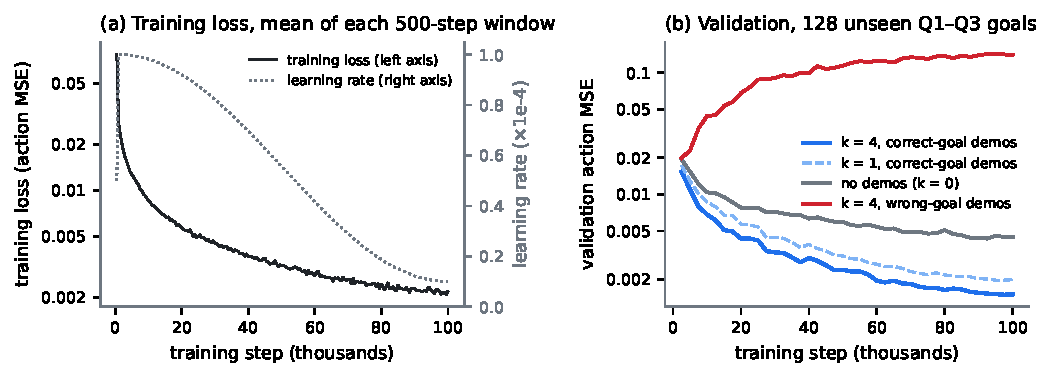
\includegraphics[width=\linewidth]{figures/fig_training.pdf}
  \caption{\textbf{Training.} (a) Training loss, the mean of each 500-step window over prompts of all $k$ (solid, left axis), and
  the learning-rate schedule (dotted, right axis). (b) Validation action MSE on 128 unseen $Q_1$--$Q_3$ goals, every 2{,}500 steps.
  Both loss axes are logarithmic because the errors span two orders of magnitude. What to notice: as the correct-goal error falls,
  the wrong-goal error \emph{rises}, so the model relies more and more on its context.}
  \label{fig:training}
\end{figure}

\subsection{In distribution, in-context control matches the teachers}
Table~\ref{tab:main} gives closed-loop success at $k = 4$. On unseen $Q_1$--$Q_3$ goals, the transformer reaches 91.2\% / 87.5\%
success-once / at-end with PPO demonstrations and 91.6\% / 87.5\% with BC demonstrations. That is within the confidence intervals
of the teachers that see the goal (94.1\% / 89.1\% and 92.0\% / 85.9\%). Under the controls it collapses: 1.4--1.6\% success-once
with wrong-goal demonstrations and 0.8--1.4\% with none. Every condition runs from the same initial states, so the gap of about
90 points is caused by the content of the context alone.

\begin{table}[h]
\centering
\caption{\textbf{Closed-loop success at $k = 4$} (\%; 512 episodes per cell, 95\% Wilson interval in brackets). One checkpoint throughout;
``Prompt'' names the teacher that recorded the demonstrations in its prompt. All conditions in a row use the same initial states.}
\label{tab:main}
\small
\begin{tabular}{lllcccc}
\toprule
Goals & Prompt & Metric & Correct goal & Wrong goal & No demos & Teacher (sees $g$) \\
\midrule
$Q_1$--$Q_3$ & PPO & once   & 91.2 [88.4, 93.4] & 1.4 [0.7, 2.8] & 1.4 [0.7, 2.8] & 94.1 [91.8, 95.9] \\
             &     & at end & 87.5 [84.4, 90.1] & 1.0 [0.4, 2.3] & 0.4 [0.1, 1.4] & 89.1 [86.1, 91.5] \\
             & BC  & once   & 91.6 [88.9, 93.7] & 1.6 [0.8, 3.1] & 0.8 [0.3, 2.0] & 92.0 [89.3, 94.0] \\
             &     & at end & 87.5 [84.4, 90.1] & 0.8 [0.3, 2.0] & 0.4 [0.1, 1.4] & 85.9 [82.7, 88.7] \\
\midrule
$Q_4$ (held out) & PPO & once   & 86.1 [82.9, 88.9] & 3.9 [2.5, 6.0] & 0.2 [0.0, 1.1] & 94.7 [92.4, 96.4] \\
                 &     & at end & 67.0 [62.8, 70.9] & 0.0 [0.0, 0.7] & 0.0 [0.0, 0.7] & 92.6 [90.0, 94.5] \\
                 & BC  & once   & 88.5 [85.4, 91.0] & 3.5 [2.2, 5.5] & 0.2 [0.0, 1.1] & 94.9 [92.7, 96.5] \\
                 &     & at end & 63.7 [59.4, 67.7] & 0.4 [0.1, 1.4] & 0.0 [0.0, 0.7] & 93.6 [91.1, 95.4] \\
\bottomrule
\end{tabular}
\end{table}

\textbf{PPO and BC prompts give the same results, by construction.} The same checkpoint, prompted with either teacher's
demonstrations, reaches the same success within the confidence intervals (Table~\ref{tab:main}, Figure~\ref{fig:k}). This says
little about generalizing across teacher types: in v1 the BC teacher is distilled from the PPO teacher, so the two produce nearly
identical demonstrations, starting from the same initial states and differing only by BC's small imitation error. We
intended PPO and BC to be distinct types of demonstrator. Testing that needs a BC teacher trained independently of PPO and a separate
learner per teacher type (Section~\ref{sec:conclusion}).

\subsection{One demonstration is nearly enough}
Figure~\ref{fig:k} varies $k$. A single demonstration already gives 90--91\% success-once on $Q_1$--$Q_3$, and $k \ge 2$ mainly
improves success-at-end (82--84\% at $k = 1$, 88\% at $k = 2$). Beyond $k = 2$ the curves are flat within their intervals. This fits
the task: the goal is a 2-D position, and one successful demonstration shows where the T ended up, which is almost the goal itself.
We return to this in Section~\ref{sec:conclusion}.
Teacher-forced error is slightly higher at $k = 8$ than at $k = 4$, which does not show in closed loop
(Appendix~\ref{app:action-error}).

\begin{figure}[h]
  \centering
  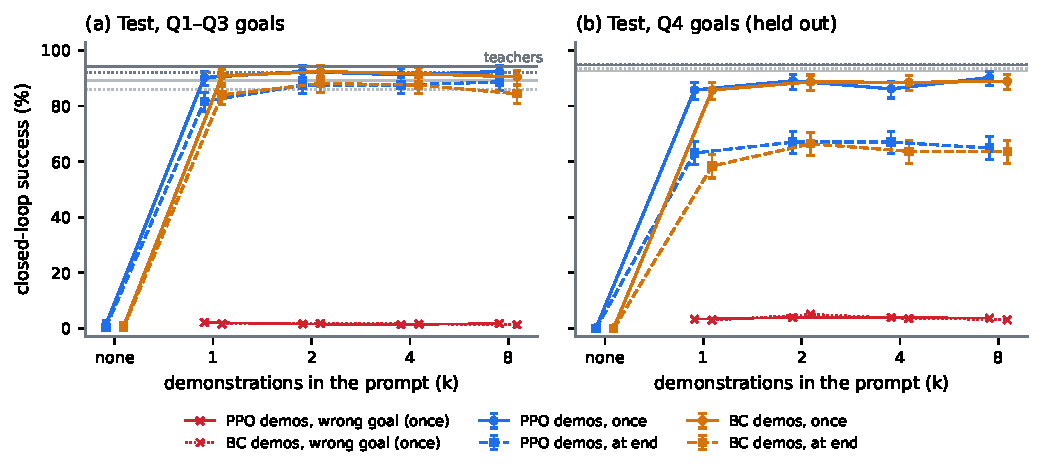
\includegraphics[width=\linewidth]{figures/fig_success_vs_k.pdf}
  \caption{\textbf{Closed-loop success vs number of demonstrations $k$} for unseen goals in $Q_1$--$Q_3$ (a) and held-out $Q_4$ goals
  (b). Colour gives the teacher that recorded the prompt (blue PPO, orange BC). Solid lines with circles show success-once and dashed
  lines with squares success-at-end, both with correct-goal demonstrations; crosses show success-once with wrong-goal demonstrations.
  The ``none'' point is the no-demonstration control. Grey lines mark the goal-seeing PPO teacher (BC teacher in Table~\ref{tab:main}).
  The $x$ axis is categorical. Error bars are 95\% Wilson intervals over 512 episodes (one training seed); PPO and BC points are offset
  slightly in $x$. What to notice: one demonstration is nearly enough, and on $Q_4$ success-at-end stays about 20--25 points below
  success-once.}
  \label{fig:k}
\end{figure}

\subsection{Held-out goals: reaching transfers, holding does not}
On $Q_4$ goals, which the transformer never trained on, the controls still behave as before: at most 3.9\% with wrong-goal
demonstrations and 0.2\% with none. The model reads held-out goals from its context. Success-once stays high (86.1--88.5\%, against
94.7--94.9\% for the teachers), but success-at-end drops to 63.7--67.0\% against the teachers' 92.6--93.6\%. In distribution, the
transformer loses about 4 points between success-once and success-at-end; on $Q_4$ it loses 19--25. This suggests that in roughly
a quarter of $Q_4$ episodes it brings the T onto the goal and then pushes it off again. We infer this from the two metrics and have
not yet inspected the trajectories. Extra demonstrations do not fix this: success-at-end
levels off at 64--67\% from $k = 2$ (Figure~\ref{fig:k}b). Teacher-forced error tells the same story: 0.0027 on $Q_4$ against 0.0016 in
distribution at $k = 4$. That is still 3$\times$ better than no context, but enough to matter for fine positioning. Our reading:
the coarse behavior, pushing toward the goal the context implies, generalizes to new goal positions. The precise corrective
actions near an unfamiliar goal do not.

\subsection{Offline error alone does not predict closed-loop success}
\label{sec:threshold}
A 3k-step pilot with the same settings reached validation action MSE 0.013 at $k = 4$, about $9\times$ the final model's, and already
preferred correct over wrong demonstrations (0.013 vs 0.016). In closed loop it scored 0\% under every condition, in a smaller
evaluation of 64 validation goals $\times$ 2 starts, while the teachers scored 91--94\% on the same starts. The final model, at
0.0015, matches the teachers. Two models are too few to locate a threshold. They do show that a model can prefer the right
demonstrations offline and still fail completely in closed loop, because small per-step errors compound over 100 steps, so
closed-loop evaluation is necessary.

\subsection{Comparison with an independent implementation}
\label{sec:compare}
One of the authors independently implemented and trained the same architecture with the same teachers, split sizes and closed-loop
protocol, in a separate codebase that collected its own demonstrations, for 50k steps at a constant learning rate in fp16 (two
seeds). Teacher success on the evaluation starts matches ours exactly, so the evaluation episodes are identical and the
closed-loop numbers are directly comparable (Table~\ref{tab:compare}). Both runs show the same qualitative results: success
comes from the context, about 0\% under both controls, $k = 1$ gives most of the effect, PPO and BC prompts give the same
results, and $Q_4$ success-at-end drops. Our run is stronger: success-once is 8 points higher and success-at-end 20 points
higher in distribution, consistent with its roughly $3\times$ lower action error.

\textbf{This comparison is not controlled.} Training length, learning-rate schedule, numeric precision and code all differ at once,
so we cannot attribute the gap to one of them. At 50k steps, the length of the independent run, our validation error was already 0.0024, below that run's
final 0.004--0.006. That suggests the decaying learning rate matters, not only the extra steps. A one-factor test is to rerun the
independent code with our schedule. Its two seeds also differ by 31 points in $Q_4$ success-at-end (41\% vs 72\%, PPO demos, $k = 4$), while
success-once is stable (77\% vs 79\%). Our single-seed $Q_4$ success-at-end therefore has wide uncertainty beyond the binomial
interval in Table~\ref{tab:main}. Success-once and the in-distribution results look stable.


% Conclusion. Part of the team paper; included by main.tex.
\section{Discussion and conclusion}
\label{sec:conclusion}

We moved the in-context learning setup of Garg et al.\ from function regression to closed-loop control, and found that a small
transformer infers a hidden goal from demonstrations well enough to match goal-seeing teachers on new goals from the training
distribution.

\textbf{What we learn.} The context acts as a strong control channel: the model follows demonstrations of the wrong goal as
confidently as the right ones. Offline error alone cannot certify a controller, so closed-loop evaluation is necessary. Out of
distribution, coarse behavior (reaching the goal) transfers before precise behavior (holding the block there).

\textbf{Did our hypotheses hold?} %CHECK: keep in sync with the hypotheses in Section 1
(i) Yes: in distribution the transformer matches the teachers, and the controls fall to 0--2\%.
(ii) Partly: reaching transfers to the held-out quadrant, but success-at-end drops by about 20--25 points, more than we expected.
(iii) No: success does not keep rising with $k$ but saturates by $k = 1$--$2$. This fits a goal that one successful demonstration
nearly reveals.
(iv) Not reliably: a pilot that already preferred correct demonstrations offline scored 0\% in closed loop. Offline error tracked
closed-loop success only once it was small.

\textbf{Limitations.} The goal is a 2-D position that a successful demonstration nearly reveals in its final state, so the
inference required is simple. We are therefore building a baseline that estimates the goal from the final T pose in the
demonstrations and gives it to the BC teacher, which will show how much more the transformer does. The main results come from one
training seed, and an independent run shows that success-at-end on held-out goals varies widely across seeds, so we are training two
more seeds to obtain between-seed error bars. Finally, v1 trains a single learner on a mixture of PPO and BC prompts, and because the
BC teacher is distilled from PPO, the two teachers implement nearly the same policy. The held-out quadrant tests
recombination more than extrapolation: each coordinate's sign appears in $Q_1$--$Q_3$, and only the combination is new. Every
demonstration and query state comes from clean teacher rollouts, so the learner never trains on the states it drifts into; Smith
et al.~\cite{smith2026transformers} found that removing state perturbations from training collapsed in-context control, which
suggests this as one cause of the holding failure on $Q_4$.

\textbf{Next steps.} v2 will treat PPO and BC policies as distinct teacher types, analogous to how Garg et al.\ train one model per
function class. We will retrain the full-state BC teacher on demonstration data in simulation instead of distilling it from PPO, so that its
behavior no longer derives from the PPO teacher. We will then train a separate transformer on each class, with the architecture,
data sizes and schedule of v1, so that only the training class changes, and evaluate each learner on its own class, on the other
class, and next to the v1 mixed learner. Three further experiments target the open questions above. Training on query states from
noisy teacher rollouts with clean labels addresses the holding failure on held-out goals. A sweep over the number of training goals
will locate where in-context generalization emerges~\cite{raventos2023pretraining}. Hidden variables that the final state does not
reveal, such as the T's mass or friction, will test inference beyond reading off the endpoint. Finally, we will repeat the study
with the camera-observation teachers.


\bibliographystyle{abbrvnat}
\bibliography{refs}

\appendix
\section{Disclosure of AI use}
\label{app:ai}
\inprogress{full disclosure of every AI tool used and what each was used for (code, literature search, writing and figures).}
% Notes for whoever writes this section (comments, not printed):
% - Claude Code (Anthropic), running Claude Opus 5.5, for the full-state BC teacher and the in-context transformer (state_bc/):
%   wrote and tested most of that code under the authors' direction (BC distillation pipeline, pusht_icl.py, Colab notebooks,
%   make_figures.py); read the logs and computed the reported numbers and intervals; drafted large parts of this report (related
%   work, method, results, conclusion) and generated the figures, all reviewed and edited by the authors; suggested and summarized
%   related work, including the Smith et al. CDC 2026 paper.
% - cs182-paper-skill (public Claude Code skill by a classmate): used with Claude Code to review the draft against the course
%   requirements, including a cold-reader test by a separate model instance that saw only the PDF.
% - Add every other tool the team used (e.g. ChatGPT, Codex, Copilot).

% Part of the team paper; included by main.tex (and by nathan_sections.tex for the standalone preview).
% ============================================================================================
\section{Teacher-forced action error}
\label{app:action-error}
\begin{table}[h]
\centering
\caption{Teacher-forced action MSE of the selected checkpoint (correct-goal / wrong-goal demonstrations; 1{,}024 prompts per cell).}
\label{tab:action-error}
\small
\begin{tabular}{lccccc}
\toprule
Split & no demos & $k{=}1$ & $k{=}2$ & $k{=}4$ & $k{=}8$ \\
\midrule
val ($Q_1$--$Q_3$) & 0.0045 & 0.0019 / 0.117 & 0.0017 / 0.128 & 0.0015 / 0.135 & 0.0017 / 0.127 \\
test ($Q_1$--$Q_3$) & 0.0044 & 0.0020 / 0.125 & 0.0017 / 0.137 & 0.0016 / 0.142 & 0.0018 / 0.134 \\
test ($Q_4$) & 0.0076 & 0.0031 / 0.077 & 0.0029 / 0.082 & 0.0027 / 0.088 & 0.0041 / 0.085 \\
\bottomrule
\end{tabular}
\end{table}
Wrong-goal error is lower on $Q_4$ because the wrong goal is another $Q_4$ goal, closer on average than goals spread over three quadrants.

\section{Development history of the BC teacher}
\label{app:teacher-history}
\inprogress{short summary of runs 1--3 from \texttt{state\_bc/README.md}. Run 1 used plain BC on released demonstrations (19\% / 10\%
success); run 2 added noisy expert rollouts and DAgger (98\% / 78\%, with DAgger adding nothing measurable); run 3 trained our own
variable-goal environment and PPO, then the team adopted the shared \texttt{PushTVarGoal-v1}.}


\section{PPO teacher and environment details}
\label{sec:ppo}
\inprogress{PPO teacher training (ManiSkill PPO baseline, 50M environment steps, seed 1, settings and training curve), the
\texttt{PushTVarGoal-v1} environment (goal sampling, quadrant layout, T and arm start distributions, success criterion), and the
per-quadrant teacher evaluation protocol: 100 episodes per quadrant with fixed seeds, and a teacher is frozen only if its
success-once is at least 80\% in every quadrant on validation episodes. Reported teacher test results: PPO 93.8\% / 91.5\% and
distilled BC 91.5\% / 88.8\% mean success-once / success-at-end, with per-quadrant numbers to be tabulated here.}

\section{Reproducibility}
\label{app:repro}
Code: \href{https://github.com/Izatr2004/icl-for-control-policies}{\texttt{github.com/Izatr2004/icl-for-control-policies}},
branch \texttt{nathan-state-bc}. %CHECK: make the repo public or add reviewers before release
The transformer is in \path{state_bc/pusht_icl.py} (subcommands \texttt{collect}, \texttt{train}, \texttt{offline},
\texttt{eval}). The Colab notebook \path{notebooks/Train_PushT_ICL_Transformer.ipynb} runs the whole pipeline on one L4 GPU
in about 4.5\,h. Every figure and table in this paper is regenerated from the committed result files, with no GPU or simulator, by
running \texttt{python}~\path{state_bc/make_figures.py}. The trained weights are in \path{state_bc/teachers/}.

\end{document}
